\documentclass[12pt, a4paper, reqno, article]{amsart}

\usepackage[]{graphicx}
\usepackage[]{hyperref}
\usepackage[]{physics}
\usepackage[]{listings}
\usepackage[utf8]{inputenc}
\usepackage[toc,page]{appendix}
%---------------------------------------------------------
\newcommand{\hbarm}{-\frac{\hbar^{2}}{2m}}
\newcommand{\ortwo}{\frac{1}{r^{2}}}
\newcommand{\ddr}{\frac{d}{dr}}
\newcommand{\ddrsq}{\frac{d^{2}}{dr^{2}}}
\newcommand{\ddrhosq}{\frac{d^{2}}{d\rho^{2}}}
\newcommand{\onehalf}{\frac{1}{2}}





\lstset{
	frame = single,
	language = C++,
	showstringspaces = false,
	tabsize = 2,
	otherkeywords = {self},
	keywordstyle = \color{blue},
	identifierstyle=\color{deepgreen},
 	stringstyle=\color{orange},
 	backgroundcolor=\color{mygray}
}

\title[Project2]{Project2: Eigenvalue problems, equations of a buckling beam,\\
  \hrulefill\small{ FYS4150: Computational Physics }\hrulefill}

\author{Sajjad Ahmadigoltapeh, Einar Aurbakken \\ Bastian Skjelstad, Per Harald Barkost}\\
%\href{https://github.com/}{\texttt{github.com}}}

\begin{document}

\begin{titlepage}
\begin{abstract}
In this project we have solved the three-dimensional Schrödinger equation for two particles with and without a repulsive Coulomb potential in a harmonic oscillator well. By discretizing the equation for one and, later, two electrons we could solve it numerically as an eigenvalue problem using the Jacobi method. By implementing the algorithm, we observe that the numerical solution coincides well with the analytical prediction. Furthermore, the only difference between the cases with and without Coulomb repulsion is the potential term, hence we can conclude that our algorithm can be modified for any potential.
\end{abstract}
\begin{center}
\tiny\url{https://github.com/einaur/fys4150/blob/master/project2/main_code/main.cpp}
\tiny\url{https://github.com/einaur/fys4150/blob/master/project2/main_code/arma_eig_solver.cpp}
\tiny\url{https://github.com/einaur/fys4150/tree/master/project2/report}
\end{center}
\maketitle
\tableofcontents
\end{titlepage}

\section{Introduction}

The aim of this study is solving an eigenvalue problem such as the buckling beam problem and the three dimensional (3D) Schrödinger equation utilizing Jacobi's method. Actually, the two-point boundary value problem of a buckling beam and the Schrödinger equation could be reformulated in a discretized form, which eventually will lead to a tridiagonal Toeplitz matrix. This matrix has analytical eigenvalues and eigenvectors, and provides a suitable condition for testing the algorithm. Furthermore, equation scaling technique is introduced in this project. In fact, making use of this technique, it is possible to define new dimensionless variables or to introduce suitable units.

\section{Theory}
Two well-known problems in physics leading to an eigenvalue problem, the \textit{Buckling beam problem} and the \textit{Schrödinger equation}, are discussed in this section.\\

\subsection{Buckling beam problem}
The buckling beam equation is given as follows:
\begin{equation}
\gamma\frac{d^2u(x)}{dx^2}=-Fu(x),
\label{eq:bbp}
\end{equation}
where $u(x)$ is the vertical displacement of the beam in the $y$ direction. The beam has length $L$, $x\in [0,L]$ and $F$ is t force applied at $(L,0)$ in the direction towards the origin. The parameter $\gamma$ is a constant defined by properties such as the rigidity of the beam. Dirichlet boundary conditions, $u(0)=u(L)=0$, are present. In the buckling beam equation, all the parameters $\gamma$, $F$ and $L$ are known. To implement scaling, a dimensional variable $\rho$ is introduced as:
\[
 \rho = \frac{x}{L},
\]
where $\rho \in [0,1]$. Then, equation (\ref{eq:bbp}) must be reformulated based on the derivative with respect to $\rho$. This means that $x$ must be replaced by $\rho$. Considering the following mathematical formula for variable change:
\[
 \frac{d^2 u}{d x^2} = \frac{d^2 u}{d \rho^2}.(\frac{d \rho}{d x})^2 + \frac{d u}{d \rho}.\frac{d^2 \rho}{d x^2},
\]
equation (\ref{eq:bbp}) may be rewritten as:
\begin{equation}
\frac{d^2 u(\rho)}{d\rho^2} = -\frac{FL^2}{R} u(\rho)=-\lambda u(\rho),
\label{eq:bbp2}
\end{equation}
where
\[
\lambda = FL^2/R.
\]\\

As shown, equation (\ref{eq:bbp}) could successfully be rewritten as equation (\ref{eq:bbp2}) after scaling, and may now be discretized. By discretization of equation (\ref{eq:bbp2}), it will be converted to an eigenvalue problem. To do so, a Taylor expansion must be used to approximate equation (\ref{eq:bbp2}) by a linear equation with $\mathcal{O}(h^2)$,
\begin{equation}
    u''=\frac{u(\rho+h) -2u(\rho) +u(\rho-h)}{h^2} + \mathcal{O}(h^2),
    \label{eq:diffoperation}
\end{equation}
where $h$ is the mesh size.
Then, the minimum and maximum values of $\rho$, $\rho_{\textrm{min}}$ and $\rho_\textrm{max}$, are given:
\[
\rho_{\mathrm{min}}=0 \hspace{0.5cm} and \hspace{0.5cm} \rho_{\mathrm{max}}=1.
\]
By a given number of mesh points, $N$, $\rho_{\mathrm{min}}$ is given by $\rho_0$ and $\rho_{\mathrm{max}}$ is given by $\rho_N$, so that $h$ will be given as
\begin{equation}
  h=\frac{\rho_N-\rho_0 }{N}.
  \label{eq:h}
\end{equation}
Therefore, the value of $\rho$ can be calculated at each point of $i$ as:
\begin{equation}
    \rho_i= \rho_0 + ih, \hspace{0.5cm}\textrm{where} \hspace{0.5cm} i=1,2,\dots , N.
    \label{eq:rhoi}
\end{equation}
By the definition in equation (\ref{eq:rhoi}), equation (\ref{eq:diffoperation}) may be rewritten as:
\begin{equation}
-\frac{u(\rho_i+h) -2u(\rho_i) +u(\rho_i-h)}{h^2}  = \lambda u(\rho_i),
\end{equation}
which leads to:
\begin{equation}
-\frac{u_{i+1} -2u_i +u_{i-1} }{h^2}  = \lambda u_i.
\label{eq:difffinal}
\end{equation}
Illustrating equation (\ref{eq:difffinal}) in matrix form gives:

\begin{equation}
    \begin{bmatrix} d& a & 0   & 0    & \dots  &0     & 0 \\
                                a & d & a & 0    & \dots  &0     &0 \\
                                0   & a & d & a  &0       &\dots & 0\\
                                \dots  & \dots & \dots & \dots  &\dots      &\dots & \dots\\
                                0   & \dots & \dots & \dots  &a  &d & a\\
                                0   & \dots & \dots & \dots  &\dots       &a & d\end{bmatrix}
                                 \begin{bmatrix} u_1 \\ u_2 \\ u_3 \\ \dots \\ u_{N-2} \\ u_{N-1}\end{bmatrix} = \lambda \begin{bmatrix} u_1 \\ u_2 \\ u_3 \\ \dots \\ u_{N-2} \\ u_{N-1}\end{bmatrix}.
\label{eq:matrixse}
\end{equation}
It is important to note that the end points, $u_0$ and $u_N$, which are subject to Dirichlet boundary conditions, are not included in equation (\ref{eq:matrixse}). In this equation, the diagonal elements, $d$, and the non-diagonal elements, $a$, are defined as
\[
d=2/h^2 \hspace{0.5cm} \textrm{and} \hspace{0.5cm} a=-1/h^2.
\]
 The eigenvalue problem presented in equation (\ref{eq:matrixse}) has analytical eigenpairs (consisting of eigenvalues and eigenvectors) given by:
\begin{equation}
\lambda_j = d+2a\cos{(\frac{j\pi}{N+1})}, \hspace{0.5cm} where \hspace{0.5cm} j=1,2,\dots, N-1.
\end{equation}
\subsection{Schrödinger equation: radial equation for single electron}
The radial part of Schrödinger's equation for a single electron in a harmonic oscillator potential is:
\begin{equation}
	\hbarm	(\ortwo \ddr r^{2} - \frac{l(l+1)}{r^{2}}) R(r) + V(r)R(r) = E R(r),
\label{eq:schrodinger}
\end{equation}

where the harmonic oscillator potential is $V(r) = \onehalf kr^{2}$, with $k = m\omega^{2}$ and $E$ being the energy of the electron and $\omega$ the oscillator frequency. Allowed energy levels are:
\begin{equation}
	E_{nl} = \hbar \omega (2n+l+\frac{3}{2}),
\end{equation}
where $n = 0,1,2,...$ is the energy quantum number and $l = 0,1,2,...$ is the orbital momentum quantum number. Assuming $R(r) = (1/r)u(r)$, equation (\ref{eq:schrodinger}) is rewritten as
\begin{equation}
	\hbarm \ddrsq u(r) + (V(r) + \frac{l(l+1)}{r^{2}}\hbarm)u(r) = Eu(r).
\label{eq:schrodingerre}
\end{equation}
By defining a dimensionless variable $\rho = (1/ \alpha)r$ equation (\ref{eq:schrodingerre}) could be scaled to equation (\ref{eq:schrodingerscaled}), where $\alpha$ is a constant with length as dimension.
\begin{equation}
	-\frac{\hbar^{2}}{2m\alpha^{2}} \ddrhosq u(\rho) + (V(\rho) + \frac{l(l+1)}{\rho^{2}}\frac{\hbar^{2}}{2m\alpha^{2}})u(\rho) = E u(\rho).
\label{eq:schrodingerscaled}
\end{equation}
To simplify the calculation, it is assumed that $l = 0$. Plugging $V(\rho) = \onehalf k\alpha^{2}\rho^{2}$ into equation (\ref{eq:schrodingerre}) gives
\begin{equation}
	-\frac{\hbar^{2}}{2m\alpha^{2}} \ddrhosq u(\rho) + \onehalf k\alpha^{2} \rho^{2}u(\rho) = E u(\rho),
\label{eq:simp}
\end{equation}
where $\frac{mk}{\hbar^{2}}\alpha^{4} = 1$ and $\lambda = \frac{2m\alpha^{2}}{\hbar^{2}}E$. By multiplying both sides of equation (\ref{eq:simp}) by
\[
2m\alpha^{2} \rho^{2} /\hbar^{2},
\]
leads to the following equation:
\begin{equation}
	-\ddrhosq u(\rho) + \rho^{2} u(\rho) = \lambda u({\rho}).
\end{equation}
To solve this equation, it should be discretized first. Using the same discretizing technique that was used in the previous section, the Schrödinger equation can be rewritten as:
\begin{equation}
  - \frac{u_{i+1}-2u_{i}+u_{i-1}}{h^{2}} + V_{i}u_{i} = \lambda u_{i}.
\label{eq:schrodingerdisc}
\end{equation}
Further simplification gives:
\begin{equation*}
  d_{i}u_{i}+e_{i-1}u_{i-1}+e_{i+1}u_{i+1} = \lambda u_{i},
\end{equation*}
where
\[
  d_{i} = \frac{2}{h^{2}} + V_{i} \hspace{1¥0.5cm} \textrm{and} \hspace{0.5cm} e_{i}= \frac{1}{h^{2}}.
\]

\subsection{Schrodinger equation: two electron in well by Coulomb interaction}
Considering two electrons in a well that are interacting with each other by repulsive Coulomb interaction, gives equation (\ref{eq:2scaled}) after scaling.
\begin{equation}
  -\frac{d^2}{d\rho^2} \psi(\rho)
       + \frac{1}{4}\frac{mk}{\hbar^2} \alpha^4\rho^2\psi(\rho)+\frac{m\alpha \beta e^2}{\rho\hbar^2}\psi(\rho)  =
\frac{m\alpha^2}{\hbar^2}E_r \psi(\rho).
\label{eq:2scaled}
\end{equation}

Defining some of the constants in equation (\ref{eq:2scaled}),
\[
\omega_r^2=\frac{1}{4}\frac{mk}{\hbar^2} \alpha^4, \hspace{0.6cm} \frac{m\alpha \beta e^2}{\hbar^2}=1, \hspace{0.6cm} \alpha = \frac{\hbar^2}{m\beta e^2} \hspace{0.3cm} \textrm{and} \hspace{0.3cm} \lambda = \frac{m\alpha^2}{\hbar^2}E,
\]
allows Schrödinger's equation to be presented as
\begin{equation}
  -\frac{d^2}{d\rho^2} \psi(\rho) + \omega_r^2\rho^2\psi(\rho) +\frac{1}{\rho} = \lambda \psi(\rho).
  \label{eq:schrodingerfinal}
\end{equation}

The general matrix form which is introduced for the dimensionless equations (\ref{eq:simp}) and (\ref{eq:schrodingerfinal}) is illustrated as:
\begin{center}
\begin{equation}
{Au} =
\begin{bmatrix}
  \frac{2}{\hbar^{2}} + V_{1} & -\frac{1}{\hbar^{2}} & 0 & \cdots & \cdots & 0 \\
  -\frac{1}{\hbar^{2}} & \frac{2}{\hbar^{2}} + V_{2} &  -\frac{1}{\hbar^{2}} & 0 &\cdots & \cdots \\
  0 & -\frac{1}{\hbar^{2}} & \frac{2}{\hbar^{2}} + V_{3} & -\frac{1}{\hbar^{2}} & 0 & \cdots \\
  \vdots & \vdots & \vdots & \vdots & \vdots & \vdots \\
  0 & \cdots & \cdots & -\frac{1}{\hbar^{2}} & \frac{2}{\hbar^{2}} + V_{N-2} & -\frac{1}{\hbar^{2}} \\
  0 & \cdots & \cdots & \cdots & -\frac{1}{\hbar^{2}} & \frac{2}{\hbar^{2}} + V_{N-1}
\end{bmatrix}
\begin{bmatrix}
	u_{1} \\
	u_{2} \\
	\vdots \\
	\\
	\\
	u_{N-1}
\end{bmatrix}
=	\lambda
\begin{bmatrix}
	u_{1} \\
	u_{2} \\
	\vdots \\
	\\
	\\
	u_{N-1}
\end{bmatrix},
\end{equation}
\end{center}

containing all the potentials of the harmonic oscillators. In the case where the harmonic oscillator potential doesn't exist, the potential terms will be \(V_{i}=\rho_{i}^{2}\). However, by considering the repulsive Coulomb potential, the total potential
becomes \(V_{i}=\omega_{r}\rho_{i}^{2}+1/\rho_{i}^{2}\), where \(\omega_{r}\) is the frequency describing the strength of the Coulomb interaction.

\subsection{Preservation of orthogonality}

The basis vectors $\vb{v}_i$ are defined as:
\begin{equation}
\vb{v}_i = \begin{bmatrix}
v_{i1} \\
\vdots \\
v_{in}
\end{bmatrix},
\end{equation}
and $\vb{v}_i$ is assumed to be an orthogonal basis,
\begin{equation}
\vb{v}_j^T\vb{v}_i=\delta_{ij}.
\end{equation}

It can be shown that for a unitary transformation $\vb{w}_i = U\vb{v}_i$, where $U$ is a unitary matrix and $U^TU=I$, the dot product and orthogonality are preserved in the unitary transformation,
\begin{align}
\vb{w}_i^T\vb{w}_j &= (U\vb{v}_i)^T  U\vb{v}_i= \vb{v}_i^TU^T U\vb{v}_j = \vb{v}_i^T I \vb{v}_j \nonumber \\
&\rightarrow \vb{w}_i^T\vb{w}_j = \vb{v}_i^T\vb{v}_j = \delta_{ij},
\end{align}
which means that dot product and orthogonality both are preserved. The necessity of this proof will be clarified in the next section. For equations of fifth order or higher there does not exist an analytical solution, however, Abel and Ruffini's theorem provides a solution for these equations utilizing iterative processes. In other words, such equations that do not have analytical solutions may be solved numerically.

\section{Algorithm}
For estimation of eigenvalues and eigenvectors of a symmetric matrix such as $A$, the Jacobi method was selected as algorithm. Using this technique, matrix $A$ is transformed to a diagonal matrix which has its eigenvalues on the diagonal.

\subsection{Jacobi's method}
The symmetric matrix $A$ is defined as:
\begin{equation}
A = \begin{bmatrix}
a_{11} & a_{12} \\
a_{21} & a_{22}
\end{bmatrix}.
\end{equation}
Since $A$ is symmetric, it is true that $a_{12}=a_{21}$. Furthermore, the rotational matrix $R$ is defined as
\begin{equation}
R = \begin{bmatrix}
\cos{\theta} & -\sin{\theta} \\
\sin{\theta} & \cos{\theta}
\end{bmatrix}.
\end{equation}
The outcome of multiplication of $R$ with any vector such as $\vb{v}$ is the rotation of the vector by an angle $\theta$. To simplify the operation, $c$ and $s$ are defined as $c=\cos{\theta}$ and $s=\sin{\theta}$, respectively. Then, similarity transforms are defined as
\begin{equation}
R^{-1}AR=\begin{bmatrix}
a_{11}c^2+2a_{12}cs + a_{22}s^2 & (a_{22}-a_{11})cs+a_{12}(c^2-s^2) \\
(a_{22}-a_{11})cs + a_{12}(c^2-s^2) & a_{11}s^2-2a_{12}s+a_{22}c^2
\end{bmatrix}.
\end{equation}
It is worth to note that the matrix of equation (\ref{eq:simp}) is a symmetric matrix. The goal of this section is rotating with $\theta$ so that the off-diagonal elements become zero. Hence we need to solve $(a_{22}-a_{11})cs + a_{12}(c^2-s^2)=0$, which gives
\begin{equation}
\tau = \cot{2\theta} = \frac{a_{11}-a_{22}}{2a_{12}}.
\end{equation}

It is possible to express all the trigonometric functions in terms of $\tau$. Setting $t = \tan{\theta}$, $c=\cos{\theta}=1/\sqrt{t^2+1}$ and $s=ct$, yields $\cot{2\theta}=1/2(\cot{\theta}-\tan{\theta}) = 1/2(2^{-1}-t)$, and finally the following quadratic equation is concluded,
\begin{equation}
t^2-2\tau t-1 =0,
\end{equation}
which has two roots. In order to ensure maximum numerical stability of these two roots, the smallest one is picked. Then, at each iteration it is rotated by a small angle.

Then relevant eigenvalues can at this point be expressed in terms of $t$ as follows:
\begin{equation}
R^{-1}AR = \begin{bmatrix}
a_{11} & 0 \\
0 & a_{22}
\end{bmatrix}.
\end{equation}
Eigenvalues are obtained by solving the characteristic equation, then by an inverse rotation of the identity matrix, eigenvectors can be obtained.

The algorithm for the $2\times2$-case is a simple example and in the case of real, practical problems, it can be extended to an $n\times n$-matrix which is called the Given's rotation matrix:
\begin{equation}
G(i,j,\theta) = \begin{bmatrix}
1 & \hdots & 0 &\hdots & 0 & \hdots & 0 \\
    \vdots & \ddots & \vdots & {} & \vdots & {} & \vdots \\
    0 & \hdots & c &\hdots & -s & \hdots & 0 \\
    \vdots & {} & \vdots & \ddots & \vdots & {} & \vdots \\
    0 & \hdots & s &\hdots & c & \hdots & 0 \\
    \vdots & {} & \vdots & {} & \vdots & \ddots & \vdots \\
0 & \hdots & 0 &\hdots & 0 & \hdots & 1
\end{bmatrix},
\end{equation}
where $s=\sin{\theta}$ and $c= \cos{\theta}$. This matrix represents a rotation in the $(i,j)$-plane with angle $\theta$. Matrix $G(k,l,\theta)$ of equation (\ref{eq:schrodingerfinal}) works as $R$ in equation (\ref{eq:2scaled}). Therefore, if matrix $A$ is multiplied by $G(i,j,\theta)^{-1}$ from the left side and by $G(k,l,\theta)$ from the right side, where $a_{kl}$ and $a_{lk}$ are equal to zero, the following system of equations is produced:

\begin{align}
\label{eq:rotation}
\begin{split}
  a^{\prime}_{hk} &= a^{\prime}_{kh} = ca_{hk} - sa_{hl}, \\
  a^{\prime}_{hl} &= a^{\prime}_{lh} = ca_{hl} - sa_{hk}, \\
  a^{\prime}_{kl} &= a^{\prime}_{lk} = (c^2 - s^2)a_{kl} + sc(a_{kk} - a_{ll}) = 0,\\
  a^{\prime}_{kk} &= c^2a^{\prime}_{kk} + s^2a_{ll} - 2sca_{kl},\\
  a^{\prime}_{ll} &= s^2a^{\prime}_{kk} + c^2a_{ll} + 2sca_{kl}.
\end{split}
\end{align}

\subsection{Algorithm implementation}
To make use of the algorithm explained above, a matrix $A$ must be made, then by applying the Jacobi method to construct a diagonalized matrix, and finally after several unit tests, it will be possible to estimate the eigenvectors.

\subsection{Making matrix $A$}
The first strategy to solve the current differential equation which is an eigenvalue problem, is to create matrix $A$. Matrix $A$ is an $n\times n$ matrix, and to be able to construct it, the elements along the diagonal must be filled.

\subsection{Diagonalizing}
The strategy in this section is to utilize symmetry transformations to force the off-diagonal elements of matrix $A$ to reach the value zero.

\section{Results and discussion}
The code was written in C++. First, the number of mesh points, $N$, was specified, and the program was executed to solve equation (\ref{eq:schrodingerdisc}). Initially, the maximum allowed difference between the lowest analytical eigenvalue and the numerical eigenvalue, $\varepsilon = \left| \lambda_{analytic}- \lambda_{num} \right|$, was set to $10^{-4}$. The lowest analytical eigenvalue is 3, and a mesh size of at least $N=200$ is required to obtain a sufficiently low value of the tolerance, $\varepsilon$. To obtain results with higher precision, the mesh size must be further increased, which in turn results in longer run times for the program.

\begin{figure}[h]
  \centering
  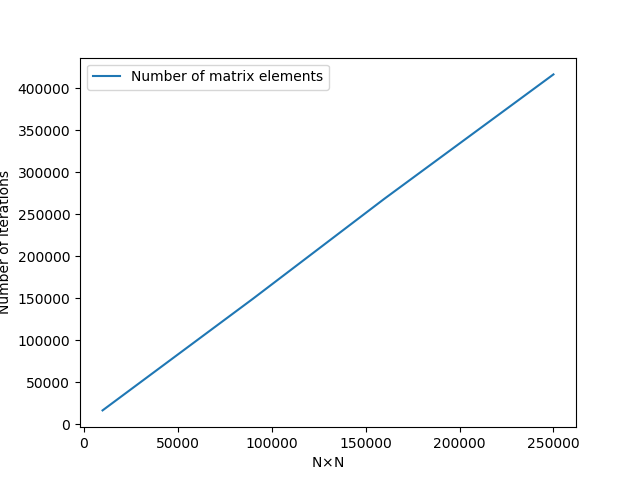
\includegraphics[width=0.8\linewidth]{iterations-vs-elements.png}
  \caption{Number of iterations as a function of number of matrix elements for $\varepsilon = 10^{-8}$.}
  \label{fig:iterations-vs-elements}
\end{figure}

By performing such transformations, it is possible to set all the non-diagonal elements to a value lower than $\varepsilon$, which approximates to zero. In this program, a counter variable is embedded to check how many times the matrix elements are rotated, the so-called number of iterations. The tolerance was at this point set to $\varepsilon = 10^{-8}$, meaning that all the off-diagonal elements would reach values lower than that of $\varepsilon$. For example, calculations were performed for a $500 \times 500$ matrix ($250\,000$ matrix elements), which resulted in approximately $400\,000$ iterations. Figure \ref{fig:iterations-vs-elements} shows the relationship between the number of matrix elements, $N \times N$, and the number of iterations. From the plot, it is evident that the relation between the number of iterations and the number of matrix elements is linear while keeping the tolerance, $\varepsilon$, constant. Therefore, in this case, if $\varepsilon$ is kept constant, the number of iterations depends solely on the matrix size.

Calculations done by the Jacobi method were compared to corresponding calculations performed by the Armadillo library in C++. The mesh size, $N$, was set to $200$ with $\varepsilon = 10^{-8}$. The run times were collected for the calculation performed by the Jacobi method and by Armadillo, and can be seen in Table \ref{tab:time}.

\begin{table}[h]
\centering
\caption{Time comparison of the Jacobi method and the Armadillo library in C++}
\label{tab:time}
\begin{tabular}{|l|l|}
\hline
\textbf{Method}  & \textbf{Time {[}s{]}} \\ \hline
Jacobi algorithm & $4.55\times{10^6}$               \\ \hline
Armadillo        & $74956$                \\ \hline
\end{tabular}
\end{table}

As can be seen from Table \ref{tab:time}, the run time is significantly longer for the Jacobi algorithm than that of Armadillo.
\\
\\

\section{Conclusion}
The solution to the Schrödinger equation for two electrons in an external harmonic oscillator was found using Jacobi's eigenvalue algorithm and the Armadillo library in C++. Compared with Armadillo, the Jacobi method is arguably slower. However, the Jacobi method is able to make the numerical eigenvalues converge to the analytical eigenvalues with great precision. Therefore, the Jacobi method is numerically stable over the working boundaries and potential in question.

\newpage

\begin{thebibliography}{9}

\bibitem{morten2}
	Hjorth-Jensen, M.,
	\emph{Project 2, Computational Physics I FYS3150/FYS4150},
	University of Oslo,
	2018.

\bibitem{abel}
	Abel, N.H.,
	Memoire sur le équations algébriques, ou l'on démontre l'impossibilité de la résolution de l'équation générale de cinquiéme degré,
	In Sylow, L. and Lie, S.,
	\emph{Æuvres Complètes de Niels Henrik Abel}, 2nd ed.,
	Grøndahl \& Søn, pp. 28-33,
	1881.

\end{thebibliography}

\begin{appendix}
\section{Laguerre Polynomials}
\label{app:laguerre}
Generally, the name Laguerre polynomials is used for solutions to
\begin{equation}
x\frac{d^2y}{dx^2}+(\alpha+1-x)\frac{dy}{dx} + ny = 0.
\end{equation}
These polynomials, usually denoted, $L_0$, $L_1$, $L_2$ etc are a polynomial sequence which may be defined by the Rodriguez formula
\begin{equation}
L_n(x) = \frac{e^x}{n!}\frac{d^n}{dx^n}(e^{-x}x^n)=\frac{1}{n!}\left(\frac{d}{dx} -1 \right)x^n.
\end{equation}



\end{appendix}

\end{document}
